%!TEX root = Slic3r-Manual.tex

If the 3D mesh described in the model contains holes, or edges are misaligned (known as being non-manifold), then Slic3r may have problems working on it.  Slic3r will attempt to fix any problems it can, but some problems are out of its reach.  If the application complains that a model cannot be sliced correctly then there are several options available, and the ones described here are all free at the time of writing.

%%% CONFIGURATION TUNING %%%
{%!TEX root = Slic3r-Manual.tex

\paragraph{Netfabb Studio} % (fold)
\label{par:netfabb_studio}
Netfabb produit une gamme d'applications de modélisation 3D, y compris une version de base gratuite\footnote{http://www.netfabb.com/basic.php}.  Cette version comprend un module de réparation de maillage qui peut aider à éliminer les différents problèmes rencontrés. Les instructions mise à jour peuvent être trouvés sur le wiki Netfabb\footnote{http://wiki.netfabb.com/Part\_Repair}, ce qui suit est un bref aperçu des étapes à suivre.

\begin{figure}[H]
\centering
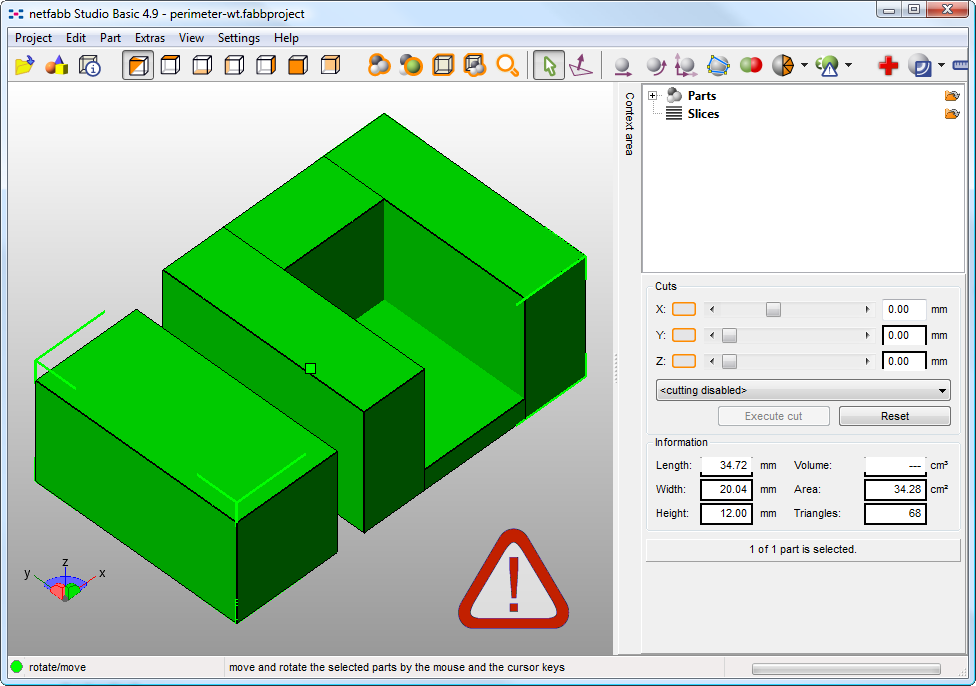
\includegraphics[keepaspectratio=true,width=0.75\textwidth]{working_with_models/netfabb_studio_part_repair.png}
\caption{Netfabb Studio: Réparation de modèle.}
\label{fig:netfabb_studio_part_repair}
\end{figure}

\begin{itemize}
	\item Lancer Netfabb studio, et charger le fichier STL qui a un problème, que ce soit par l'intermédiaire du menu \texttt{File} ou par glisser-déposer sur l'espace de travail. Si Netfabb détecte un problème, il affiche un signe d'alerte rouge dans le coin en bas à droite.
	\item Pour exécuter les scripts de réparation, sélectionnez la partie et puis cliquez sur la première icône d'aide dans la barre d'outils (la croix rouge), ou sélectionnez dans le menu contextuel \texttt{Extras->Repair Part}.  Cela va ouvrir l'onglet réparation de modèle et de montrer l'état du modèle.
	\item Les onglets \texttt{Actions} et \texttt{Repair scripts} offrent plusieurs scripts de réparation qui peuvent être appliquées manuellement, mais dans le but de cet aperçu sélectionez le script \texttt{Automatic repair} corrigera la plupart des problèmes.
	\item Le bouton de réparation automatique présente deux options: par défaut et simples. Choisir par défaut couvrira la plupart des cas. Selectionnez \texttt{execute} pour lancer le script.
	\item Une fois la pièce réparée les réparations doivent être appliquées en sélectionnant \texttt{Apply repair}, choisissant s'il faut passer outre la partie existante ou non.
	\item La pièce peut ensuite être exporté en sélectionnant \texttt{Export part->As STL} à partir du menu contextuel.
	\item Si Netfabb détecte encore que la partie exportée contient des erreurs, alors il offrira la possibilité d'appliquer d'autres réparations avant de l'exporter.
	\begin{figure}[H]
	\centering
	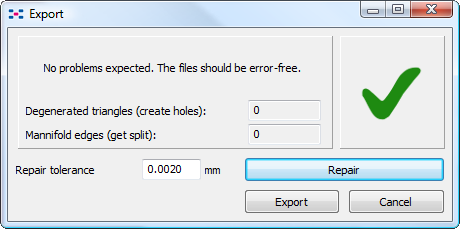
\includegraphics[keepaspectratio=true,width=0.75\textwidth]{working_with_models/netfabb_studio_export_part.png}
	\caption{Netfabb Studio: Export de pièce.}
	\label{fig:netfabb_studio_export_part}
	\end{figure}
\end{itemize}
% paragraph netfabb_studio (end)

\paragraph{Netfabb Cloud Service} % (fold)
\label{par:netfabb_cloud_service}
Netfabb accueille également un service web où un fichier STL peut être téléchargé pour être vérifié et réparé\footnote{http://cloud.netfabb.com/}.  

\begin{figure}[H]
\centering
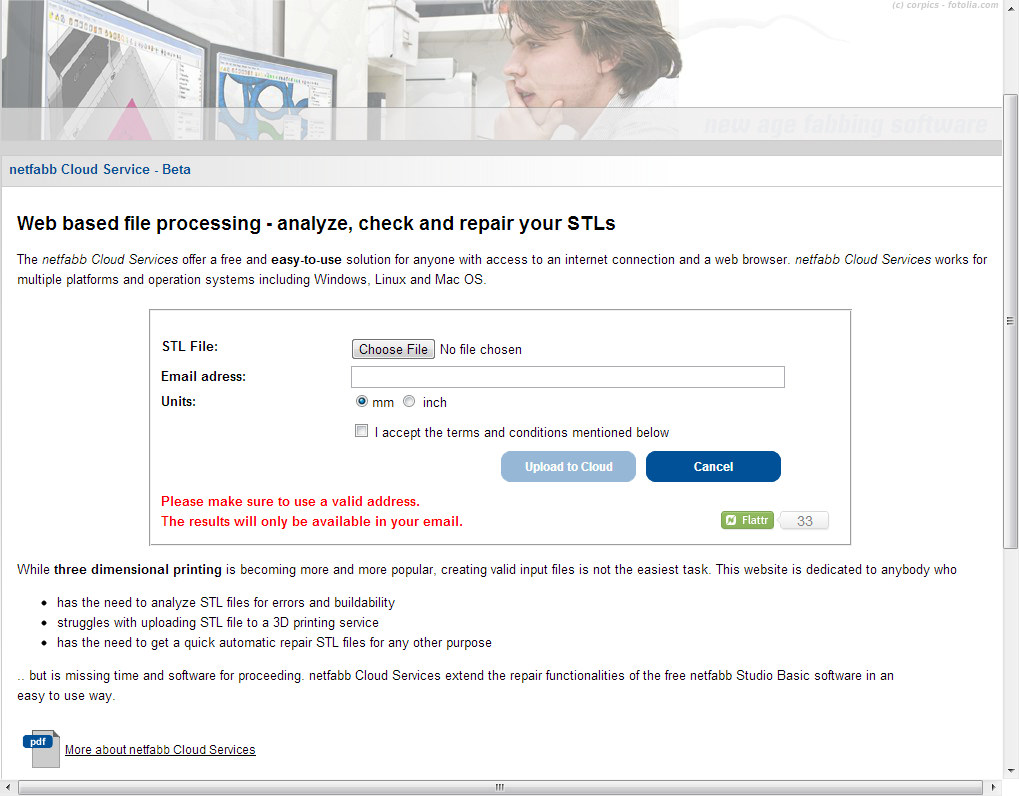
\includegraphics[keepaspectratio=true,width=0.75\textwidth]{working_with_models/netfabb_cloud_services.png}
\caption{Netfabb Cloud Services.}
\label{fig:netfabb_cloud_services}
\end{figure}

\begin{itemize}
	\item Accédez à http://cloud.netfabb.com
	\item Choisissez le fichier STL à télécharger en utilisant le bouton prévu.
	\item Une adresse e-mail doit être donnée pour vous informer quand la prestation est terminé.
	\item Choisissez entre les mesures métriques ou impériales qui doivent être utilisés.
	\item Lisez et acceptez les conditions de service, puis cliquez sur \texttt{Upload to Cloud}.
	\item Une fois que le service a analysé et réparé le fichier, un email est envoyé, fournissant le lien de téléchargement du fichier réparé.
\end{itemize}
}
%%% END CONFIGURATION TUNING %%%

\paragraph{FreeCAD} % (fold)
\label{par:freecad}
\index{FreeCAD}

Freecad\footnote{\url{http://sourceforge.net/projects/free-cad}} is a comprehensive, and free, CAD program which comes with a mesh module, in which repairs to degenerate models can be made.  the following steps outline how a problem model file can be analysed and repaired.

\begin{figure}[H]
\centering
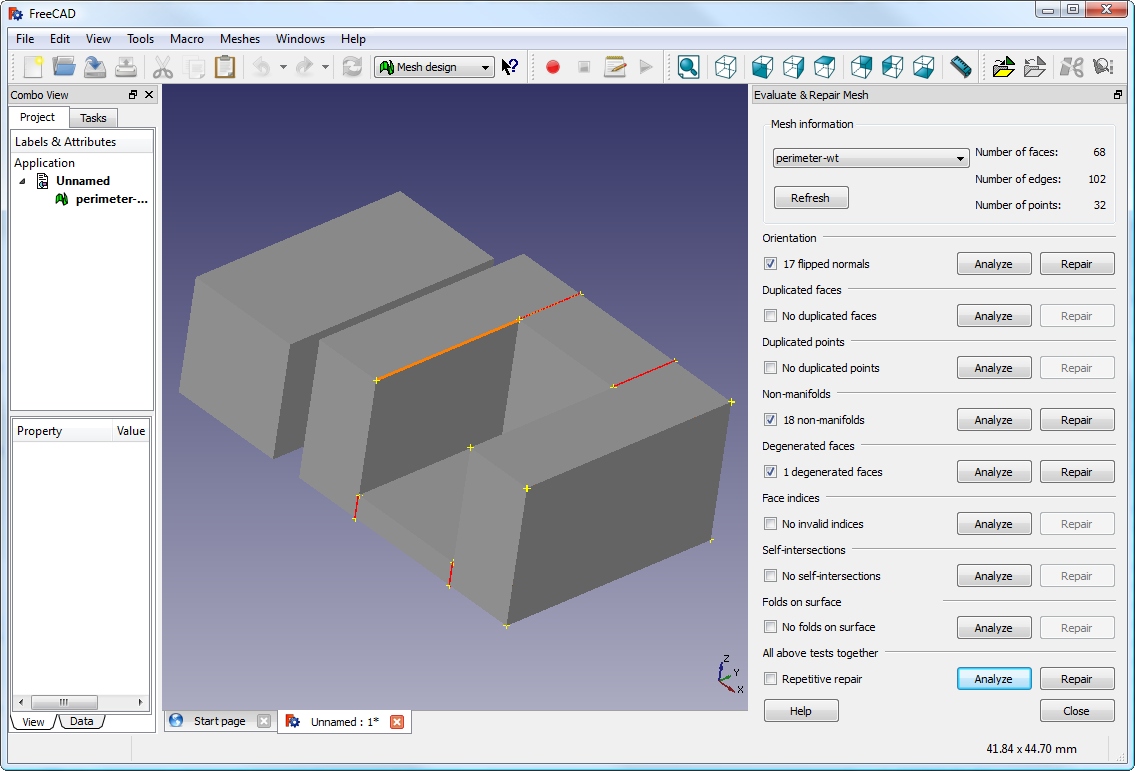
\includegraphics[keepaspectratio=true,width=0.75\textwidth]{working_with_models/freecad_part_repair.png}
\caption{FreeCAD part repair.}
\label{fig:freecad_part_repair}
\end{figure}

\begin{itemize}
	\item Start FreeCAD and from the start splash page choose \texttt{Working with Meshes}.
	\item Load the model by dragging and dropping it onto the workspace or via the \texttt{File} menu.  A small message in the bottom left corner will indicate if the model appears to have problems.
	\item From the menu choose \texttt{Meshes->Analyze->Evaluate \& Repair mesh} to bring up the repair options dialog.
	\item From the options dialog choose the loaded mesh, then perform each analysis be clicking the \texttt{Analyze} button by each problem type, or select \texttt{Repetitive Repair} at the bottom to perform all checks.  If a corresponding problem is detected the \texttt{Repair} button becomes enabled.
	\item For each desired repair hit the \texttt{Repair} button.
	\item It is important to review the effect the repair script has made to the model.  It may be the case that the script damages the file, rather than repair, for example by removing important triangles.
	\item Export the repaired model via the \texttt{Export} menu option or context menu.
\end{itemize}
% paragraph freecad (end)
